%%%%%%%%%%%%%%%%%%%%%%%%%%%%%%
% 生物統計のまとめ
%%%%%%%%%%%%%%%%%%%%%%%%%%%%%%

\part{生物統計学}

\chapter{生物統計学:基本}

生物統計学の基本を扱う.

\section{理解度チェックリスト}

生物統計学の基本の理解度チェックリスト\cite{キホンのキ}を以下に示した.

\begin{itemize}
  \item 基本
        \begin{todolist}
          \item 記述統計学と推測統計学の違いは?
          \item 母集団を意識して研究しているか?(研究者の基本)
          \item 母集団と標本の違いは?
          \item 母数とは?
          \item 統計量とは?
          \item 3 種類の標準偏差の違いは?
          \begin{itemize}
            \item 母標準偏差(母分散)
            \item 標本標準偏差(標本分散)
            \item 不偏標準偏差(不偏分散)
          \end{itemize}
        \end{todolist}
  \item 標本分布,推定,検定
        \begin{todolist}
          \item 標本分布とは?
          \item 標準偏差(SD)と標準誤差(SE)はどう違うか?
          \item SD と SE はそれぞれどんな意図を持って用いられるか?
          \item 正規性の検定,糖分酸性の検定は何のためにあるのか?必要か?
          \item パラメトリック検定,ノンパラメトリック検定とは何か?どう使い分ける?
          \item 対応のある(関連した)検定と対応のない(独立した)検定はどう違うのか?\footnote{対応のある検定 paired test,対応のない検定 unpaired test}
          \item 片側検定,両側検定はどう違うのか?
          \item 有意差とはどう言う意味か?どのようにして有意差を決めるのか?
          \item 帰無仮説,対立仮説,危険率,有意水準の意味とは?
        \end{todolist}
  \item 分散分析,実験計画
        \begin{todolist}
          \item 一元配置分散分析で何が分かるのか?
          \item 3 群以上ではなぜ t 検定ではなく,多重比較なのか?
          \item 二元配置分散分析で何が分かるのか?どのような実験に使えるのか?
          \item どうすれば有意差の得られやすい実験計画が立てられるのか?
          \item 実験計画の立案に統計の知識はどうかかわるのか?
        \end{todolist}
\end{itemize}

\section{標準偏差の種類}

母標準偏差・・・母集団の平均からのずれ(ばらつき)を表す値.

\[
  \sigma = \sqrt{\frac{\Sigma(x_i - \mu)^2}{N}}
\]

標本標準偏差・・・標本の平均からのずれ(ばらつき)を表す値.

\[
  s = \sqrt{\frac{\Sigma(x_i - \bar{x})^2}{n}}
\]

不偏標準偏差・・・母標準偏差を推定するための値.

\[
  u = \sqrt{\frac{\Sigma(x_i - \bar{x})^2}{n-1}}
\]

\section{標本平均の分布}

母集団が $N(\mu, \sigma^2)$ から標本抽出を行った時,サンプルサイズを $n$,各観測値を $X_i$,観測値の平均値を $\bar{X}$,とする.各観測値は独立とする.

各観測値は $N(\mu, \sigma^2)$ に従うため,以下のように表せる.

\begin{eqnarray}
  X_1 \sim N(\mu, \sigma^2)\\
  X_2 \sim N(\mu, \sigma^2)\\
  \vdots\\
  X_n \sim N(\mu, \sigma^2)
\end{eqnarray}

各観測値は独立であるため,以下が成り立つ.

\begin{eqnarray}
  X_1 + X_2 + \cdots + X_n & \sim & N(\mu + \mu + \cdots + \mu, \sigma^2 + \sigma^2 + \cdots + \sigma^2)\\
  X_1 + X_2 + \cdots + X_n & \sim & N(n\mu, n\sigma^2)(「観測値の和」が従う確率分布)
\end{eqnarray}

上記より,標本平均 $\bar{X}$ の従う分布が導ける.

\begin{eqnarray}
  \frac{X_1 + X_2 + \cdots + X_n}{n} & \sim & N(\mu, \frac{\sigma^2}{n})(\because V(c X) = c^2 V(X))\\
  \bar{X} & \sim & N(\mu, \frac{\sigma^2}{n})
\end{eqnarray}

\newpage

\subsection{補足:期待値,分散の性質}

標本平均の従う分布を導く際に利用した期待値の性質をまとめておく.

\begin{itemize}
  \item 期待値
        \begin{eqnarray}
          E(X) & = & \sum_{i=1}^{n} x_i f(x)(離散型)\\
          E(X) & = & \int_{-\infty}^{\infty} x f(x)(連続型)
        \end{eqnarray}
  \item 期待値の演算
        \begin{equation}
          \begin{aligned}
            E(c)     & = c(定数)                     \\
            E(X + c) & = E(X) + c                      \\
            E(cX)    & = c E(X)(期待値のスカラー倍)  \\
            E(X + Y) & = E(X) + E(Y)(期待値の加法性)
          \end{aligned}
        \end{equation}
\end{itemize}

続いて分散の性質を列挙する.

\begin{itemize}
  \item 分散
        \begin{eqnarray}
          V(X) & = & E\{(X - \mu)^2\}(定義)\\
          V(X) & = & \sum_{i=1}^{n} (x_i - \mu)^2 f(x)(離散型)\\
          V(X) & = & \int_{-\infty}^{\infty} (x - \mu)^2 f(x)(連続型)
        \end{eqnarray}
  \item 分散の定義から導かれる性質
        \begin{eqnarray}
          V(X) = E(X^2) - (E(X))^2
        \end{eqnarray}

        証明
        \begin{eqnarray*}
          \begin{aligned}
            V(X) & = E\{(X - \mu)^2\}(\because 分散の定義)                                      \\
                 & = E(X^2 - 2\mu X + \mu^2)(\because 展開)                                     \\
                 & = E(X^2) - 2\mu E(X) + E(\mu^2)(\because 期待値の加法性,期待値のスカラー倍) \\
                 & = E(X^2) - 2\mu^2 + \mu^2(\because E(X) = \mu,定数の期待値)                 \\
                 & = E(X^2) - \mu^2                                                               \\
                 & = E(X^2) - (E(X))^2    (\because E(X) = \mu,定数の期待値)                   \\
          \end{aligned}
        \end{eqnarray*}
  \item 分散の演算
        \begin{eqnarray}
          \begin{aligned}
            V(c)     & = 0        \\
            V(X + c) & = V(X)     \\
            V(c X)   & = c^2 V(X)
          \end{aligned}
        \end{eqnarray}
        証明 $V(c X) = c^2 V(X)$
        \begin{eqnarray}
          \begin{aligned}
            V(c X) & = E\{(cX - E(cX))^2\}(\because 分散の定義 V(X) = E\{(X - E(X))^2\}) \\
                   & = E\{(cX - cE(X))^2\}(\because 期待値のスカラー倍)                  \\
                   & = E\{c^2(X - E(X))^2\}                                                \\
                   & = c^2 E\{(X - E(X))^2\}(期待値のスカラー倍)                         \\
                   & = c^2 V(X)(\because 分散の定義 E\{(X - E(X))^2\} = V(X))            \\
          \end{aligned}
        \end{eqnarray}
\end{itemize}

\section{標本平均の分布による区間推定}

前節では,標本平均 $\bar{X}$ が従う分布を求めることができた.これにより,「標本平均の」標準偏差が $\frac{\sigma}{\sqrt{n}}$ であることが分かった.
この「標本平均の分散」のように,ある母集団から標本抽出を行い,その観測値から得た\textbf{統計量のばらつきを標準偏差で表したもの}を「\textbf{標準誤差 standard error(SE)}」という.\\

統計量を指定せずに単に「標準誤差」と言った場合,\textbf{「標本平均の」標準誤差 stardard error of the mean(SEM)}のことを指す.

\begin{itemize}
  \item 標準誤差・・・統計量のばらつきを標準偏差で表したもの.統計量を指定せずに単に「標準誤差」と行った場合,標本平均の標準偏差(標本平均の「標準誤差」)を表すことが多い.
\end{itemize}

ここでは,標準誤差を「標本平均の標準誤差」として扱う.標準誤差は標本平均の標準偏差であるため,

\begin{itemize}
  \item 区間 $\mu \pm 1 SE$・・・標本抽出を行って標本平均を算出した時,$67 \%$ の確率でその区間に収まる
  \item 区間 $\mu \pm 1.96 SE$・・・標本抽出を行って標本平均を算出した時,$95 \%$ の確率でその区間に収まる
\end{itemize}

\newpage

\section{正規分布のグラフの概形}

正規分布 $N(\mu, \sigma^2)$ に従う母集団\footnote{正規分布に従う母集団を「正規母集団」という}から以下の条件で標本抽出を行った場合を考える.

\begin{itemize}
  \item $N(\mu, \sigma^2) = N(50, 20^2)$
        \begin{itemize}
          \item 母平均 50,母標準偏差 20(母分散 400)
        \end{itemize}
  \item サンプル数:10\footnote{サンプル数 the number of samples・・・群数,サンプルの数(\textbf{「サンプル = 群」と覚えておけば間違えない.}).詳しくは「\linedhref{https://biolab.sakura.ne.jp/sample-size.html}{サンプル数とサンプルサイズは意味が違う}」を参照.「サンプル」の誤用として多いのが,「個々の測定値(観測値)をサンプルと思っている」である.}
  \item サンプルサイズ:30\footnote{サンプルサイズ sample size・・・1 サンプルの大きさ.}
\end{itemize}

\begin{figure}[H]
  \begin{center}
    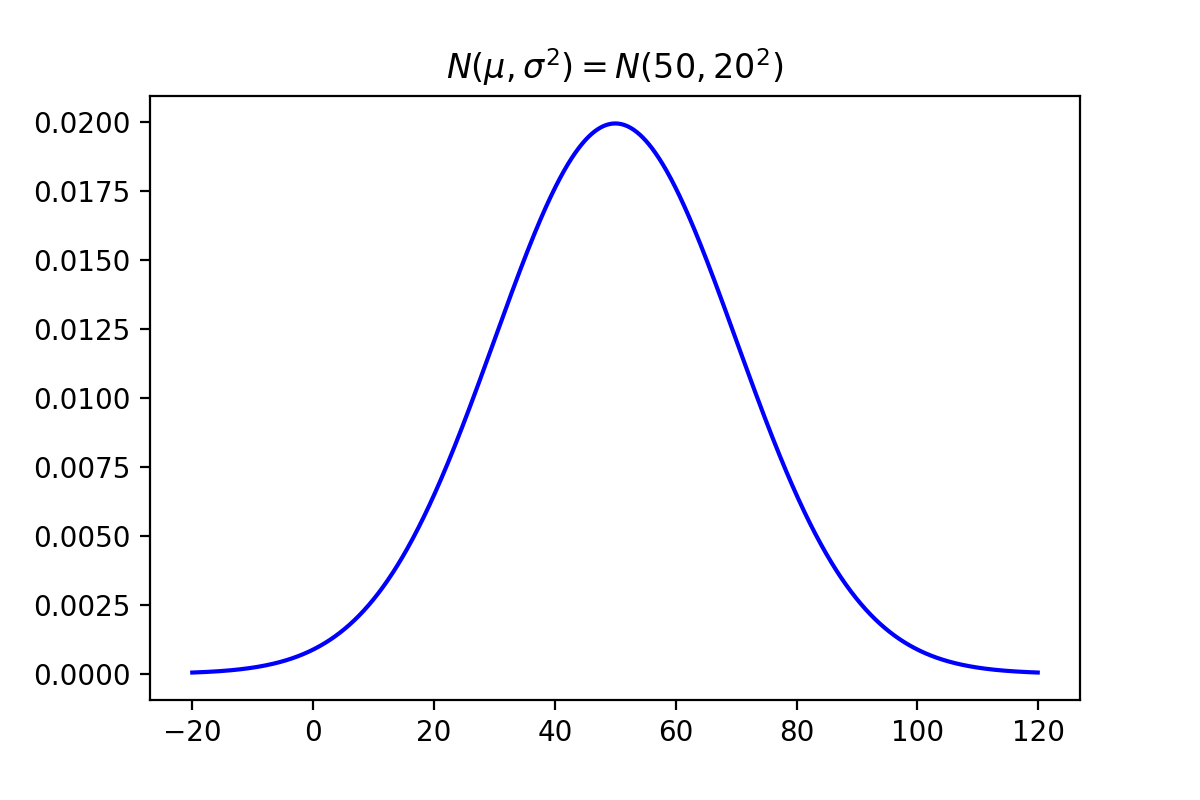
\includegraphics[width=15cm]{images/parts/3/norm-dist.png}
    \caption{$N(\mu, \sigma^2) = N(50, 20^2)$ の正規分布}
  \end{center}
\end{figure}

一つのサンプルを $X_i = \{x_1, x_2, \ldots, x_{30}\}$ としたとき,

\section{パラメトリック検定,ノンパラメトリック検定}
\section{2 群間比較の統計手法}
\section{3 群感比較の統計手法}

\chapter{生物統計学:応用}
\section{多変量解析}
\section{クラスタリング}
\section{主成分分析}

\chapter{オミクス解析}
\section{オミクス解析の基本的な流れ}
\section{トランスクリプトーム}
\subsection{Enrichment 解析}
基本,「発現が上がっている遺伝子と下がっている遺伝子の組」という発想が Enrichment 解析の精神.
「(有意に)上がっている,下がっている」をどう決めるかは関連分野の論文を参考にして定める,もしくは独自の指標で定める.

\subsection{Enrichment 解析の注意点}

GO(Gene Ontology)によって大規模データの Enrichment 解析をする時,多重検定補正をしてもなお,
補正後 p-value(q-value)は実際より高めに見積もられてしまう.
これは,各々の遺伝子に割り当てられた annotation term が重複してる場合があるためである.

「重複を免れない」というデータ構造上の問題まできちんと明示的に考えて Enrichment 解析を使ってる生物系の論文ってあまり見ない気がする.
もちろん,予め有意水準低めに設定して検定を厳しくするとかはできる.

\subsection{メタボローム}
